\section{Faserbündel}
\label{sec:faserbundel}

\begin{figure}[t]
  \begin{tikzpicture}[MyPersp]%,font=\large]
    % the base circle is the unit circle in plane Oxy
    \def\h{1.5}% Heigth of the ellipse center (on the axis of the cylinder)
    \def\offa{0.5}% 
    \def\offb{2.6}%
    \def\offc{1.4}%
    \def\offd{3}%

    %%%%%%%%%%%%%%%%%%%%%
    % representation of E
    %%%%%%%%%%%%%%%%%%%%%
    \foreach \t in {10,20,...,360}% generatrices 1
      \draw[dashed] ({\offb*cos(\t)},{\offc*sin(\t)},0)--({\offb*cos(\t)},{\offc*sin(\t)},{2.0*\h});
    \draw[very thick] (\offb*1,\offc*0,0) % lower circle
	\foreach \t in {5,10,...,360}{--({\offb*cos(\t)},{\offc*sin(\t)},0)}--cycle;
    \draw[very thick] (\offb*1,\offc*0,{2*\h}) % upper circle
	\foreach \t in {5,10,...,360}{--({\offb*cos(\t)},{\offc*sin(\t)},{2*\h})}--cycle;
	
    \fill[] (-1.5,0,2*\h) circle (0pt) node[left]{$E$}; 
	
    %%%%%%%%%%%%%%%%%%%%%
    % representation of B, U and x
    %%%%%%%%%%%%%%%%%%%%%
    \draw[very thick] (\offb*1,\offc*0,{3*\h}) % B
	\foreach \t in {5,10,...,360}{--({\offb*cos(\t)},{\offc*sin(\t)},{3*\h})}--cycle;
    \draw[magenta, very thick] ({1+\offa},{0},{3*\h}) % U
	\foreach \t in {5,10,...,360}{--({cos(\t)+\offa},{sin(\t)},{3*\h})}--cycle;
    
    \fill[]     (-1.5,0,3*\h) circle (0pt) node[left]{$B$}; 
    \fill[magenta] (1,0,3*\h) circle (0pt)node[right]{$U$};
    \fill[blue]	 (0,0,3*\h) circle (1pt)node[left]{$x$};
    
  %   \draw[<-,thick] (-1.5,0,3*\h)--(-1.5,0,2*\h) node[above right]{$\pi$};
    \draw[<-,thick] (-1.5,0,3*\h)--(-1.5,0,2*\h);
    \fill[] (-1.5,0,2.5*\h) circle (0pt)node[right]{$\pi$};
    
    %%%%%%%%%%%%%%%%%%%%%
    % representation of pi^-1(U)
    %%%%%%%%%%%%%%%%%%%%%
    \foreach \t in {20,40,...,360}% generatrices
      \draw[magenta, dashed] ({cos(\t)+\offa},{sin(\t)},0)--({cos(\t)+\offa},{sin(\t)},{2.0*\h});
    \draw[magenta, very thick] ({1+\offa},{0},0) % lower circle
	\foreach \t in {5,10,...,360}{--({cos(\t)+\offa},{sin(\t)},0)}--cycle;
    \draw[magenta, very thick] ({1+\offa},{0},{2*\h}) % upper circle
	\foreach \t in {5,10,...,360}{--({cos(\t)+\offa},{sin(\t)},{2*\h})}--cycle;
	
    \draw[blue, very thick] (0,0,0) -- (0,0,2*\h) node[left]{$E_x$};
  %   \fill[blue] (0,0,\h) circle (0pt) node[left]{$\pi^{-1}(x)$};
    
    %%%%%%%%%%%%%%%%%%%%%
    % representation of UxF
    %%%%%%%%%%%%%%%%%%%%%
    \foreach \t in {20,40,...,360}% generatrices
      \draw[orange, dashed] ({cos(\t)-\offd},{sin(\t)+\offd},0)--({cos(\t)-\offd},{sin(\t)+\offd},{2.0*\h});
    \draw[orange, very thick] ({1-\offd},{0+\offd},0) % lower circle
	\foreach \t in {5,10,...,360}{--({cos(\t)-\offd},{sin(\t)+\offd},0)}--cycle;
    \draw[orange, very thick] ({1-\offd},{0+\offd},{2*\h}) % upper circle
	\foreach \t in {5,10,...,360}{--({cos(\t)-\offd},{sin(\t)+\offd},{2*\h})}--cycle;
	
    \draw[red, very thick] (0-\offd,0+\offd,0) -- (0-\offd,0+\offd,2*\h);
    \fill[red]    (0-\offd,0+\offd,\h) circle (0pt) node[right]{$F$};
    \fill[orange] (0-\offd,0+\offd,2*\h) circle (0pt) node[left]{$U \times F$}; 
    
    %%%%%%%%%%%%%%%%%%%%%
    % representation of Phi_U
    %%%%%%%%%%%%%%%%%%%%%
    \draw[->,thick] (-0.5,0.5,\h) -- (-2.2,2.2,\h) node[above left]{$\Phi_U$};

  \end{tikzpicture}
  \caption{Skizze eines Faserbündels.}
  \label{fig:faserbundel}
\end{figure}

\thmbox{defn}{Faserbündel}{\label{def:faserbundel}Seien $E$, $B$, $F$ \difmans, $\pi \colon E \to B$ eine glatte surjektive Funktion.\\
Falls es um jeden Punkt $x \in B$ eine Umgebung $U$ sowie einen Diffeomorphismus $\Phi_U \colon \pi^{-1}(U) \to U \times F$ gibt, sodass 
\begin{equation}
\pi_U \after \Phi_U = \pi
\label{eq:kommut}
\end{equation}
gilt, nennen wir $\left( E, \pi, B\right)\footnotemark = \left( E, \pi, B ; F\right)$ \textbf{Faserbündel} mit \textbf{typischer Faser} $F$. \footnotetext{Diese kürzere Schreibweise findet Verwendung,
wenn $F$ klar oder nicht relevant ist.}
Nach \autoref{eq:kommut} kommutiert also folgendes Diagramm:
\begin{center}
  \begin{tikzpicture}[->, >=stealth', shorten >=1pt, auto, node distance=2.8cm, semithick]
    \tikzstyle{every state}=[draw=none]

    \node[state] (A)			{$\pi^{-1}(U) \subset E$};
    \node[state] (B) [below right of=A]	{$U \subset B$};
    \node[state] (C) [above right of=B] {$U \times F$};

    \path (A) edge              node {$\Phi_U$} (C)
	      edge              node {$\pi$} (B)
	  (C) edge              node {$\pi_U$} (B);
  \end{tikzpicture}
\end{center}%\\
$B$ heißt \textbf{Basisraum} und $E$ \textbf{Totalraum} des Faserbündels. Die Abbildung $\Phi_U$ wird auch \textbf{lokale Trivialisierung} oder \textbf{Bündelkarte} genannt.
Mit $E_x := \pi^{-1}(x)$  bezeichnen wir für alle $x \in B$ die \textbf{Faser} über $x$. }

\begin{wrapfigure}{R}{0.40\textwidth}
  \centering
  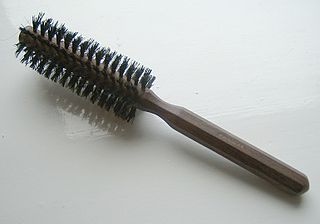
\includegraphics[width=0.40\textwidth]{roundhairbrush.jpg}
  \caption[Alltagsbeispiel eines Faserbündels: Runde Haarbürste.]{Alltagsbeispiel eines Faserbündels: Runde Haarbürste.\footnotemark}
  \label{fig:hairbrush}
\end{wrapfigure}

\autoref{fig:faserbundel} veranschaulicht die Komponenten aus \hyperref[def:faserbundel]{Definition }\ref{def:faserbundel}. Neben der Beziehung zwischen dem Totalraum $E$ und dem Basisraum $B$ 
sind in blau ein Punkt $x \in B$ und sein Urbild $E_x$ bezüglich $\pi$ sowie in magenta die Umgebung $U$ um $x$ und deren Urbild unter $\pi$ dargestellt. Zudem sind die typische Faser $F$ in rot 
und der Diffeomorphismus $\Phi_U$ sowie dessen Bild $U \times F$ in orange abgebildet.

Ein Beispiel aus dem Alltag, das als Faserbündel aufgefasst werden kann, ist eine Haarbürste, wie sie in \autoref{fig:hairbrush} abgebildet ist. Der Basisraum $B$ ist der Holzzylinder, der 
Totalraum $E$ sind die Borsten. Die lokale Trivialisierung $\pi$ bildet jeden Punkt der Borsten auf ihre jeweilige Wurzel auf dem Zylinder ab.\footnotetext{Quelle: https://upload.wikimedia.
org/wikipedia/commons/thumb/c/ca\-/Round\-hair\-brush.JPG/\-320px-Roundhairbrush.JPG}\footnote{Dieses Beispiel wurde auf https://en.wikipedia.org/wiki/Fiber\_bundle gefunden.}

\thmbox{defbem}{}{\label{thm:defbem}Für jede lokale Trivialisierung $\Phi_U$ und alle $x \in U$ sei folgende Abbildung definiert: \[\Phi_{U,x} \colon E_x \to F , \ \Phi_{U,x} := \pi_F \after \Phi_U.\] 
Dann ist für jede Faser $E_x$ durch $\Phi_{U,x}$ ein Isomorphismus auf die typische Faser $F$ gegeben, daher auch der Name.}

\thmbox{defn}{Isomorphie}{Seien $( E, \pi, B)$ und $( \tilde E, \tilde \pi, B )$ Faserbündel über dem gleichen Basisraum $B$. Wir nennen die Faserbündel isomorph, falls
es einen Diffeomorphismus $\Psi \colon E \to \tilde E$ gibt, sodass $\tilde \pi \after \Psi = \pi$. Schematisch gilt also Folgendes:
\begin{center}
  \begin{tikzpicture}[->, >=stealth', shorten >=1pt, auto, node distance=2.8cm, semithick]
    \tikzstyle{every state}=[draw=none]

    \node[state] (A)			{$E$};
    \node[state] (B) [below right of=A]	{$B$};
    \node[state] (C) [above right of=B] {$\tilde E$};

    \path (A) edge              node {$\Psi$} (C)
	      edge              node {$\pi$} (B)
	  (C) edge              node {$\tilde \pi$} (B);
  \end{tikzpicture}
\end{center}}%

\thmbox{bsp}{}{Seien $M$ und $F$ \difmans, $\pi \colon M \times F \to M$ die Projektion auf die erste Komponente. Dann ist $(M \times F, \pi, M; F)$ ein Faserbündel.
Jedes zu diesem Faserbündel isomorphe Faserbündel nennen wir \textbf{trivial}. \cite{baum}}

\thmbox{bsp}{}{Sei $M$ eine n-dimensionale \difman. Die folgenden Bündel sind Faserbündel mit Basisraum $M$ \cite{baum}:
\begin{enumerate}
 \item das Tangentialbündel: $\left( TM, \pi, M; \R^n \right)$,
 \item das Cotangentialbündel: $\left( T^* M, \pi, M; \R^n \right)$,
 \item das k-Formenbündel: $\left( \Omega^k M, \pi, M; \R^{\binom{n}{k}} \right)$.
\end{enumerate}
}

\thmbox{bsp}{}{Sei $(B,g)$ eine n-dimensionale Riemannsche Mannigfaltigkeit. Setze: 
\begin{align*}
  E   &:= \{ x \in TB \ | \ \norm{x}_g = 1 \},\\
  \pi &:= {\pi_{_{TB}}\big|}_E.
\end{align*}
Das Faserbündel $(E,\pi,B)$ heißt \textbf{Einheits-Sphären-Bündel}.

Dieser Name leitet sich von der typischen Faser $F = S^{n-1}$ her. Dies folgt, da mit den Definitionen von $E$ und $\pi$ für alle $p \in B$ gilt: 
\[ \pi^{-1}(p) = \{ x \in T_pB \ | \ \norm{x}_g = 1 \}.\]
Die lokalen Trivialisierungen erhält man aus denen des Tangentialbündels. \cite{baer} 
}

\subsection{Cozykeln}

Seien $(E, \pi, B ; F)$ ein Faserbündel und $\mathfrak{U} = \{U_i\}_{i \in I}$ eine offene Überdeckung von $B$ mit zugehörigen lokalen Trivialisierungen 
$\mathfrak{T} = \{ \Phi_U \}_{U \in \mathfrak{U}}$. 
Für $U_i,U_k \in \mathfrak{U}$ und $\Phi_{U_i}, \Phi_{U_k} \in \mathfrak{T}$ erhält man durch Hintereinanderausführung die sogenannten \textbf{Übergangsfunktionen}:
\[
  \Phi_{U_i} \after \Phi_{U_k}^{-1} \colon (U_i \cap U_k) \times F \to (U_i \cap U_k) \times F.
\]
Durch die in \hyperref[thm:defbem]{Definition und Bemerkung }\ref{thm:defbem} definierten Abbildungen erhält man aus den Übergangsfunktionen für $(i,k) \in I^2$ Abbildungen
\[
  \Phi_{ik} \colon U_i \cap U_k \to \text{Diff}(F), \ x \mapsto \Phi_{U_i,x} \after \Phi_{U_k,x}^{-1}.
\]

\thmbox{defn}{Cozykeln}{Die zuvor konstruierten Abbildungen $\{ \Phi_{ik} \}_{i,k \in I}$ heißen \textbf{Cozykeln des Fa\-ser\-bün\-dels}.}

\thmbox{lemdef}{Cozykelbedingung}{Die Cozykeln $\{ \Phi_{ik} \}_{i,k \in I}$ eines Faserbündels $(E, \pi, B; F)$ erfüllen für alle $i,j,k \in I$ folgende Eigenschaften:
\begin{align*}
  &\text{1. } & \Phi_{ik} \cdot \Phi_{kj} &= \Phi_{ij}& \\
  &\text{2. } & \Phi_{ii} &= \text{id}_F& \\
\end{align*}
Dies wird die \textbf{Cozykelbedingung} genannt. 
}

\subsection{Konstruktionen}

\thmbox{lemdef}{Rückzug}{\label{def:ruck} Seien $M, N$ \difmans, und $f \colon N \to M$ eine glatte Abbildung. Für ein Faserbündel $(E, \pi, M)$ definieren wir $f^*(E, \pi, M) := (f^*E, \tilde \pi, N)$ durch:
\begin{align*}
  f^*E &:= \{ (y,e) \in N \times E \ | \ f(y) = \pi(e) \}\\
  \tilde \pi(y,e) &:= y
\end{align*}
Damit ist $(f^*E, \tilde \pi, N)$ ein Faserbündel über $N$ und heißt der \textbf{Rückzug} (engl.: pull back) von $(E, \pi, M)$ entlang $f$. Dabei bleibt die typische Faser erhalten.
Ein Beweis wird von \textcite{baum} geführt.}

\thmbox{bem}{}{Sei $F$ eine glatte Mannigfaltigkeit und $\varphi \colon F \to F$ ein Diffeomorphismus. Dann wirkt $\Z$ durch $(k, (t,f)) \mapsto (t+k, \varphi^k(f))$ eigentlich diskontinuierlich auf 
$\R \times F$.

Mit $E := \fak{\R \times F}{\Z}$ und $\pi \colon E \to \fak{\R}{\Z} \cong S^1 =: B$ ist $(E, \pi, B)$ ein Faserbündel mit typischer Faser $F$. \cite{baer}}

Geometrisch wird der Totalraum $E$ also aus den trivialen Bündeln $[0,1] \times F \to [0,1]$ durch ``Zusammenkleben'' der Fasern durch den Diffeomorphismus $\varphi$ konstruiert.
Um lokale Trivialisierungen zu konstruieren, nutzt man die (globale) Trivialität der Projektion $\pi_\R \colon \R \times F \to \R$ sowie die eigentliche Diskontinuität der Wirkung. \cite{baer}

\subsection{Schnitte}

\thmbox{defn}{Schnitt}{Unter einem glatten Schnitt eines Faserbündels $(E, \pi, B)$ versteht man eine glatte Abbildung $s \colon B \to E$, sodass $\pi \after s = id_B$. Mit $\Gamma(E)$ bezeichnen
wir die Menge aller Schnitte in $E$.}

\thmbox{defbem}{Vektorbündel}{Für ein beliebiges Faserbündel $(E, \pi, B ; F)$ kann für die Menge der Schnitte $\Gamma(E) = \emptyset$ gelten.

Existiert jedoch ein Isomorphismus $F \to \K^n$, $\K \in \{ \R, \C \}$, so gibt es immer Schnitte (vgl. \hyperref[bem:null]{Bemerkung }\ref{bem:null}). 
Ein solches Faserbündel nennen wir auch \textbf{$\K$-Vektorbündel von Rang $n$}.}

\thmbox{bem}{Nullschnitt}{\label{bem:null} Sei $(E, \pi, B ; F)$ ein Vektorbündel. Dann existiert wegen der Isomorphie zu $K^n$ ein eindeutiges Element $0_F$. Damit kann der sogenannte 
\textbf{Nullschnitt} wie folgt definiert werden:
\[s_0(x) := 0_F \text{ , für alle } x \in B.\]
Es gilt also $s_0 \in \Gamma(E) \neq \emptyset$.}

\thmbox{bem}{}{Für ein triviales Faserbündel $(M \times F, \pi_M, M)$ gilt offensichtlich:
\[\Gamma(M \times F) = \mathcal{C}^\infty(M,F)\]
Weitere bekannte Objekte aus der Geometrie, die als Schnitte von Vektorbündeln aufgefasst werden können sind \cite{baer}:
\begin{table}[!h]
  \centering
  \begin{tabular}{c|c}
    Vektorbündel & Schnitte\\
    \hline
    $TB$ & Vektorfelder über $B$\\
    $T^*B$ & 1-Formen über $B$\\
    $\Omega^k T^*M$& k-Formen über $B$\\
  \end{tabular}
\end{table}}